\section{Calibrações}


\begin{frame}{Calibrações necessárias}
    
    \begin{itemize}
        \item<1-> 2 calibrações intrínsecas:
            \begin{itemize}
                \item<3-> Calibração câmara
                \item<4-> Calibração do laser
            \end{itemize}
        \item<2-> 2 calibrações extrínsecas:
            \begin{itemize}
                \item<5-> Calibração Câmara-PTU - \textit{Hand to Eye Calibration}
                \item<6-> Calibração Câmara-Laser - \textit{RADLOCC Calibration}
            \end{itemize}
    \end{itemize}

\end{frame}

\subsection{Hand2Eye Calibration}


\begin{frame}{Descrição Hand2Eye Calibration}

    \begin{itemize}
        
        \item Algoritmo de calibração de uma câmara em relação a um braço robotizado através de um algoritmo regressor.
        \item Utiliza um marcado de fácil identificação e estimação de pose por visão), como um ARuCo, como um objeto estático.
        \item Existem dois pares de transformações conhecidas e desconhecidas, usadas como \textit{inputs} para o regressor.
        \item Algoritmo implementado na biblioteca VISP e também disponível no ROS.

    \end{itemize}    

\end{frame}

\begin{frame}{Fórmula}

    \centering
    \begin{tikzpicture}
        
        \node[draw, ellipse] at (0, 0) (Base) {Base};
        \node[draw, ellipse] at (2, 2) (Hand) {Hand};
        \node[draw, ellipse] at (4, 4) (Camera) {Camera};
        \node[draw, ellipse] at (8, 1) (Object) {Object};

        \draw[->] (Base) edge node[auto, color=blue] {$T_{Base}^{Hand}$} (Hand);
        \draw[->] (Hand) edge node[auto, color=red] {$T_{Hand}^{Camera}$} (Camera);
        \draw[->] (Camera) edge node[auto, color=blue] {$T_{Camera}^{Object}$} (Object);
        \draw[->] (Base) edge node[auto, color=red] {$T_{Base}^{Object}$} (Object);
    \end{tikzpicture}

    $$T_{Base}^{Hand} \cdot T_{Hand}^{Camera} \cdot T_{Camera}^{Object} = T_{Base}^{Object}$$

\end{frame}

\begin{frame}{Procedimento}
    
    \begin{enumerate}
        \item Movimento do braço robótico (PTU).
        \item Identificação da pose do marcado através da imagem da câmara. 
        \item Registo das 2 transformações.
        \item Voltar ao primeiro passo até registar poses suficientes.
        \item Correr o algoritmo regressor.
    \end{enumerate}

\end{frame}

\begin{frame}{Teste}

    Para testar a qualidade da calibração encontrada podem-se utilizar as seguintes técnicas:

    \begin{itemize}
        \item O algoritmo de calibração tem como resultado um erro associado ao \textit{dataset} de \textit{input}.
        \item Um marcado pode ser usado novamente para avaliar o sistema. Num sistema calibrado, o marcado deverá manter-se na mesma posição após um movimento do braço (PTU).
        \item Esta avaliação poderá ser feita inicialmente visualmente ou mais corretamente, registando posições do marcador sucessivamente e de seguida calculado o desvio nessa amostra.
    \end{itemize}
    
\end{frame}

\subsection{RADLOCC}

\begin{frame}{Calibração Câmera-Laser}

    Este algoritmo consiste num otimizador chamado RADLOCC que cruza dados de uma câmara e de um laser para encontrar a transformação entre os dois.

    É usado um \textit{chessboard} como marcador, por ser possível estimar a pose nas imagens da câmara e por servir como alvo para o laser.

    Influencia especialmente no registo de cor.
    
\end{frame}

\begin{frame}{Algoritmo}

    \centering
    \begin{tikzpicture}
        
        \node[draw, ellipse] (Images) {Imagens};
        \node[draw, rectangle, below of=Images, yshift=-0.5cm] (PEstimation) {Estimativa de Pose};
        \node[draw, ellipse, below of=PEstimation, yshift=-0.5cm] (Poses) {CB Poses};
        
        \node[draw, ellipse, right of=Images, xshift=3cm] (LaserScans) {LaserScans};
        \node[draw, rectangle, below of=LaserScans, yshift=-0.5cm] (Segmentation) {Segmentação};
        \node[draw, ellipse, below of=Segmentation, yshift=-0.5cm] (Points) {CB Points};

        \node[draw, rectangle, below of=Points, yshift=-0.5cm] (Transformation) {Transformação};
        \node[draw, ellipse, right of=Transformation, xshift=2cm] (TF) {TF};
        \node[draw, rectangle, below of=Poses, yshift=-0.5cm] (Projection) {Projeção};
        \node[draw, ellipse, below of=Projection, yshift=-0.5cm] (Error) {Erro};

        \draw[->] (Images) edge (PEstimation);
        \draw[->] (PEstimation) edge (Poses);
        \draw[->] (Poses) edge (Projection);
        \draw[->] (Projection) edge (Error);

        \draw[->] (LaserScans) edge (Segmentation);
        \draw[->] (Segmentation) edge (Points);
        \draw[->] (Points) edge (Transformation);
        \draw[->] (TF) edge (Transformation);
        \draw[->] (Transformation) edge (Projection);


    \end{tikzpicture}
    
\end{frame}

\begin{frame}{Dataset}

    É necessário registar várias \textit{Imagens} e \textit{LaserScans}.

    É necessário conter variação suficiente nas poses do \textit{Chessboard} para que o algoritmo possa convergir.

    É necessário que o fundo seja estático, para que a segmentação seja fácil.

\end{frame}

\begin{frame}{Teste}
    
    Como teste da calibração da calibração existem vários métodos:

    \begin{itemize}
        \item Reprojeção dos pontos do laser nas imagens do dataset.
        \item Reprojeção dos pontos do laser em \textit{realtime}.
        \item Análise do registo da cor nas nuvens de pontos das capturas.
    \end{itemize}

\end{frame}

\begin{frame}{Má reprojeção dos pontos}
    
    \centering
    \begin{figure}
        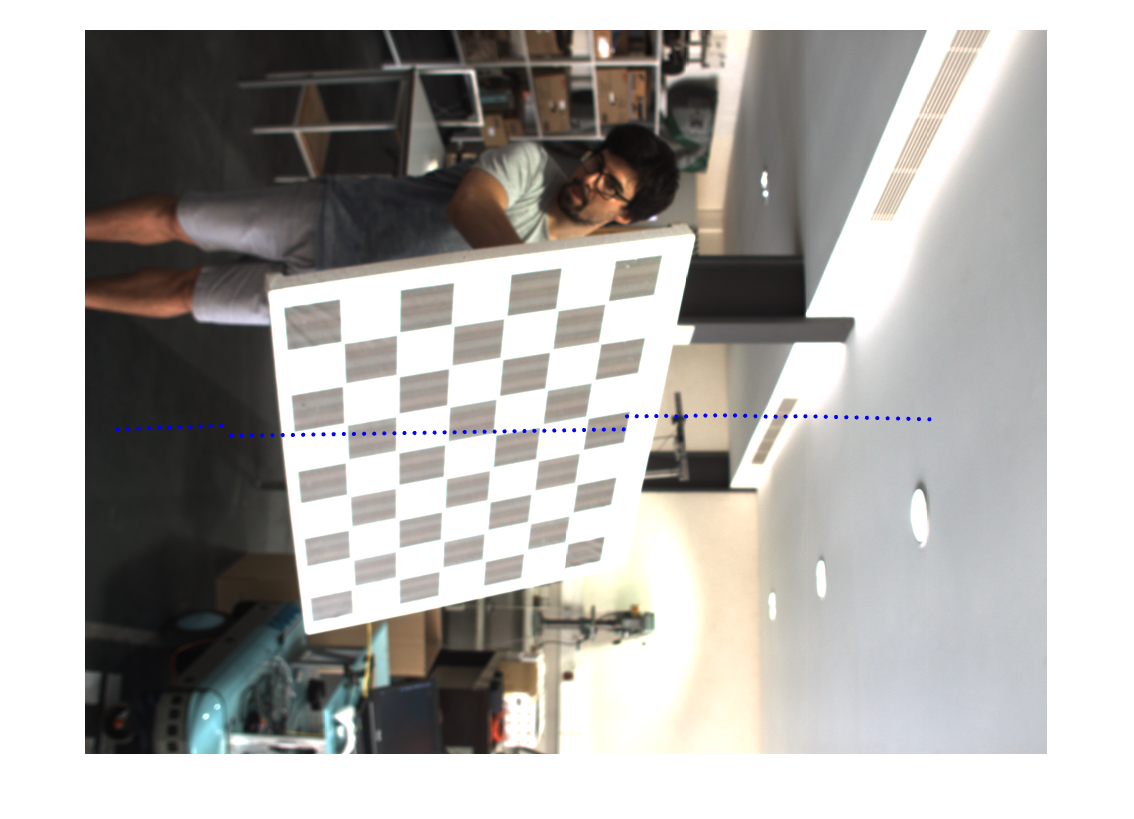
\includegraphics[angle=90, width=0.6\textheight]{img/radlocc_bad_calibration.png}
    \end{figure}

\end{frame}

\begin{frame}{Boa reprojeção dos pontos}

    \centering
    \begin{figure}
        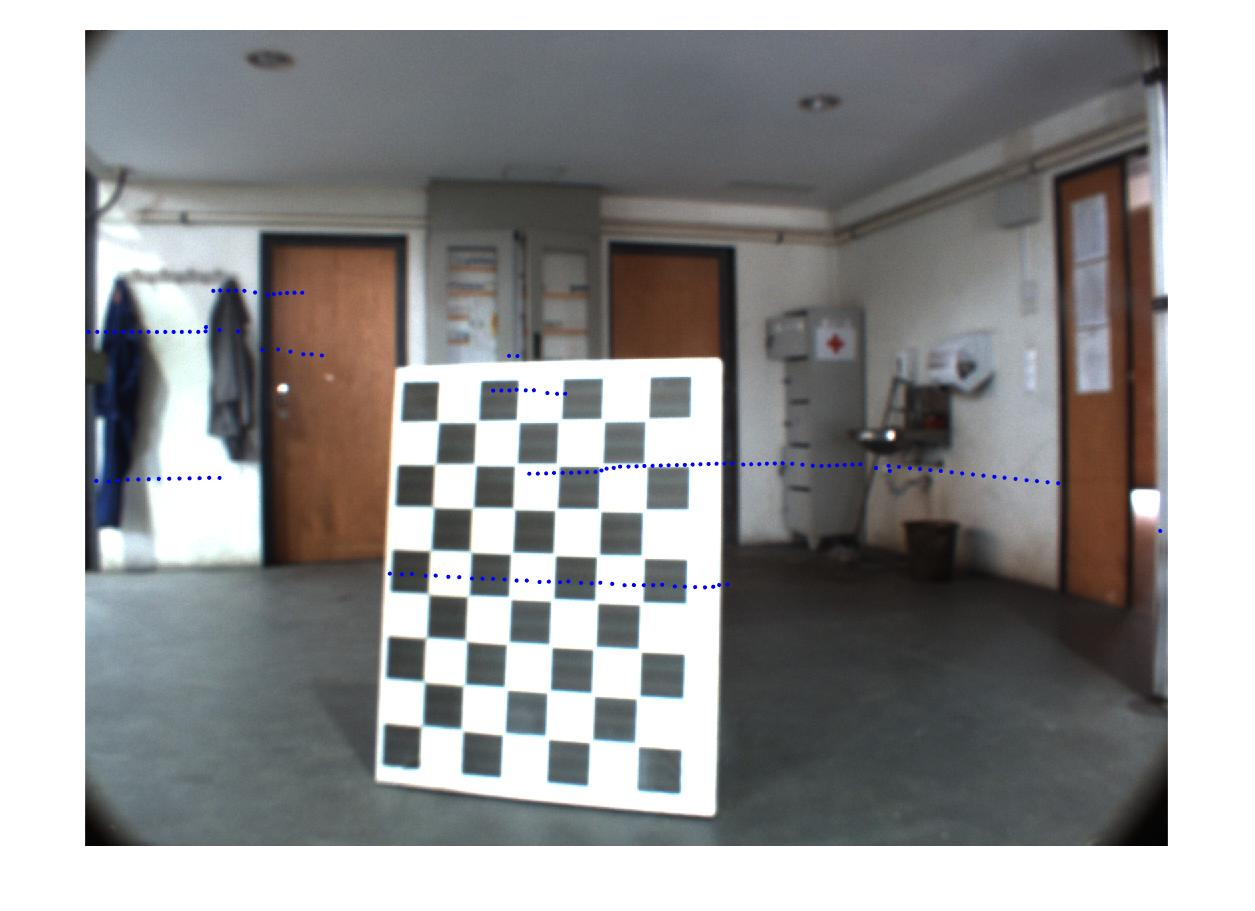
\includegraphics[width=\textwidth]{img/radlocc_good_calibration.jpg}
    \end{figure}

\end{frame}

\begin{frame}{Mau registo na acquisição}
    
    \centering
    \begin{figure}
        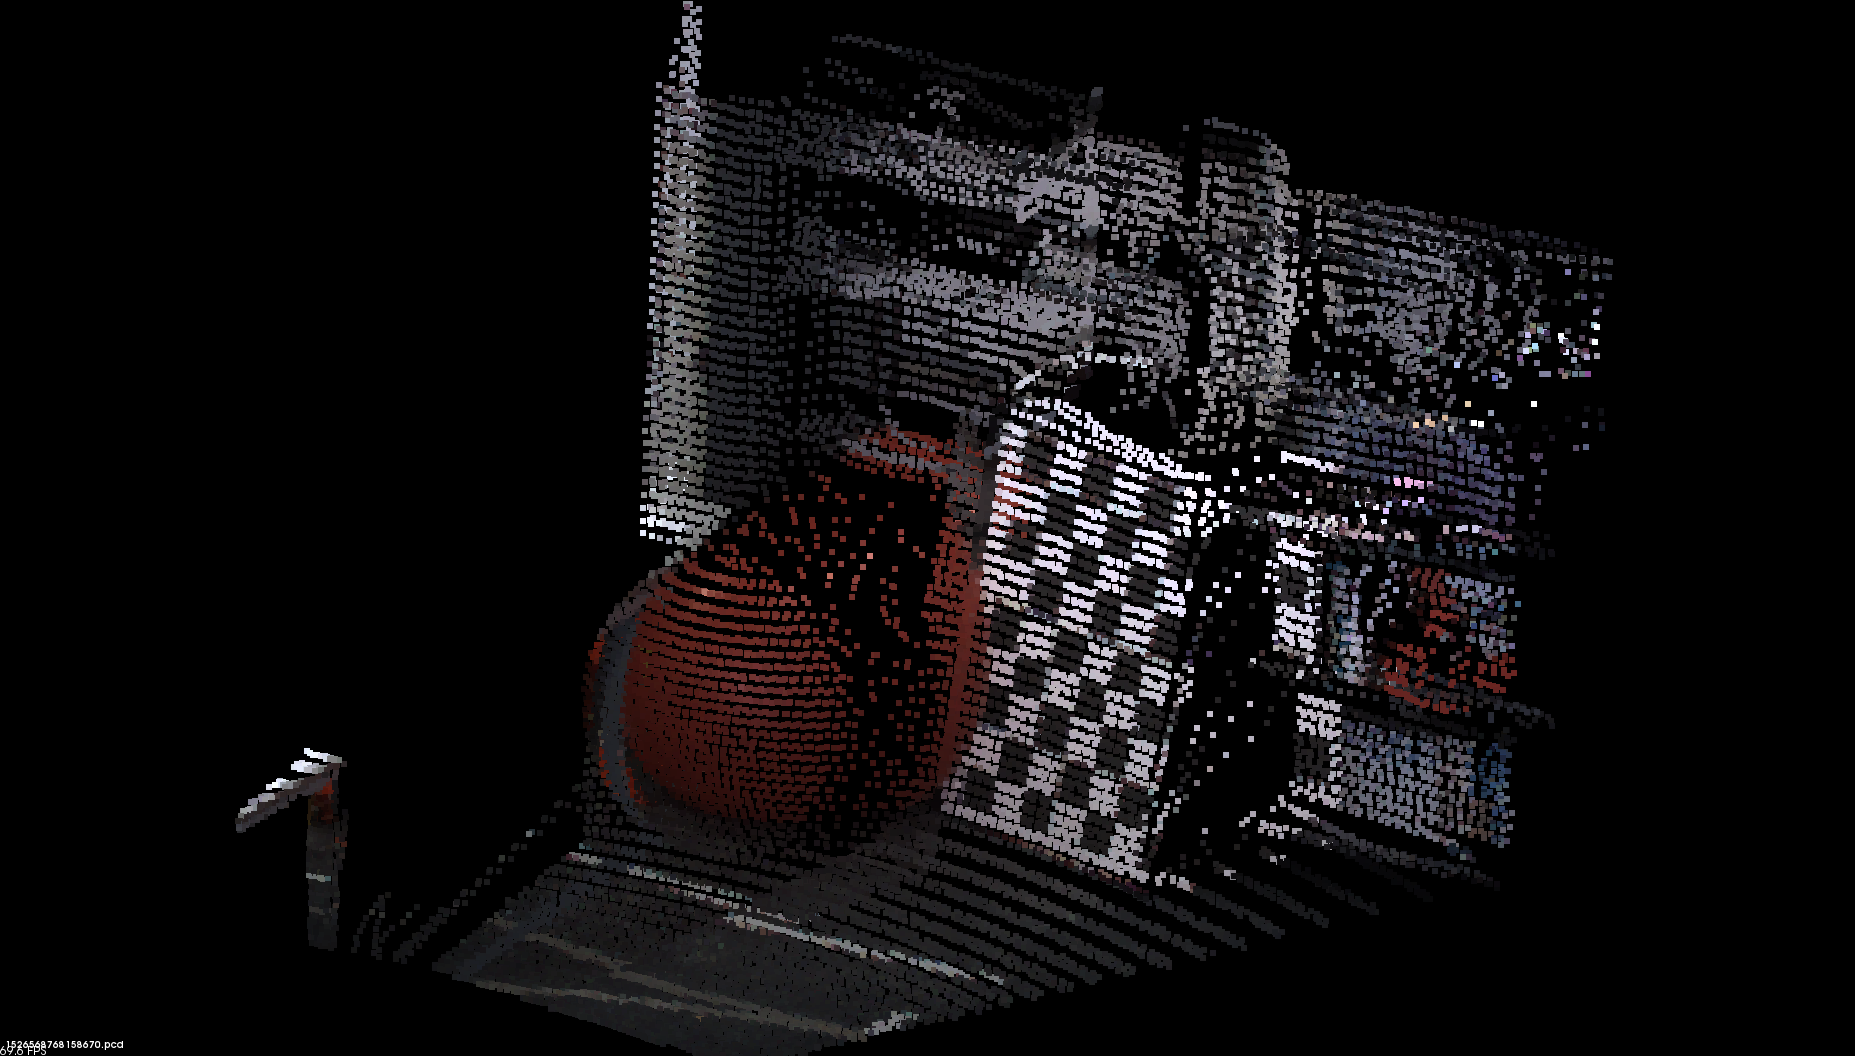
\includegraphics[width=\textwidth]{img/radlocc_bad_regist.png}
    \end{figure}

\end{frame}

\begin{frame}{Melhor registo na acquisição}
    
    \centering
    \begin{figure}
        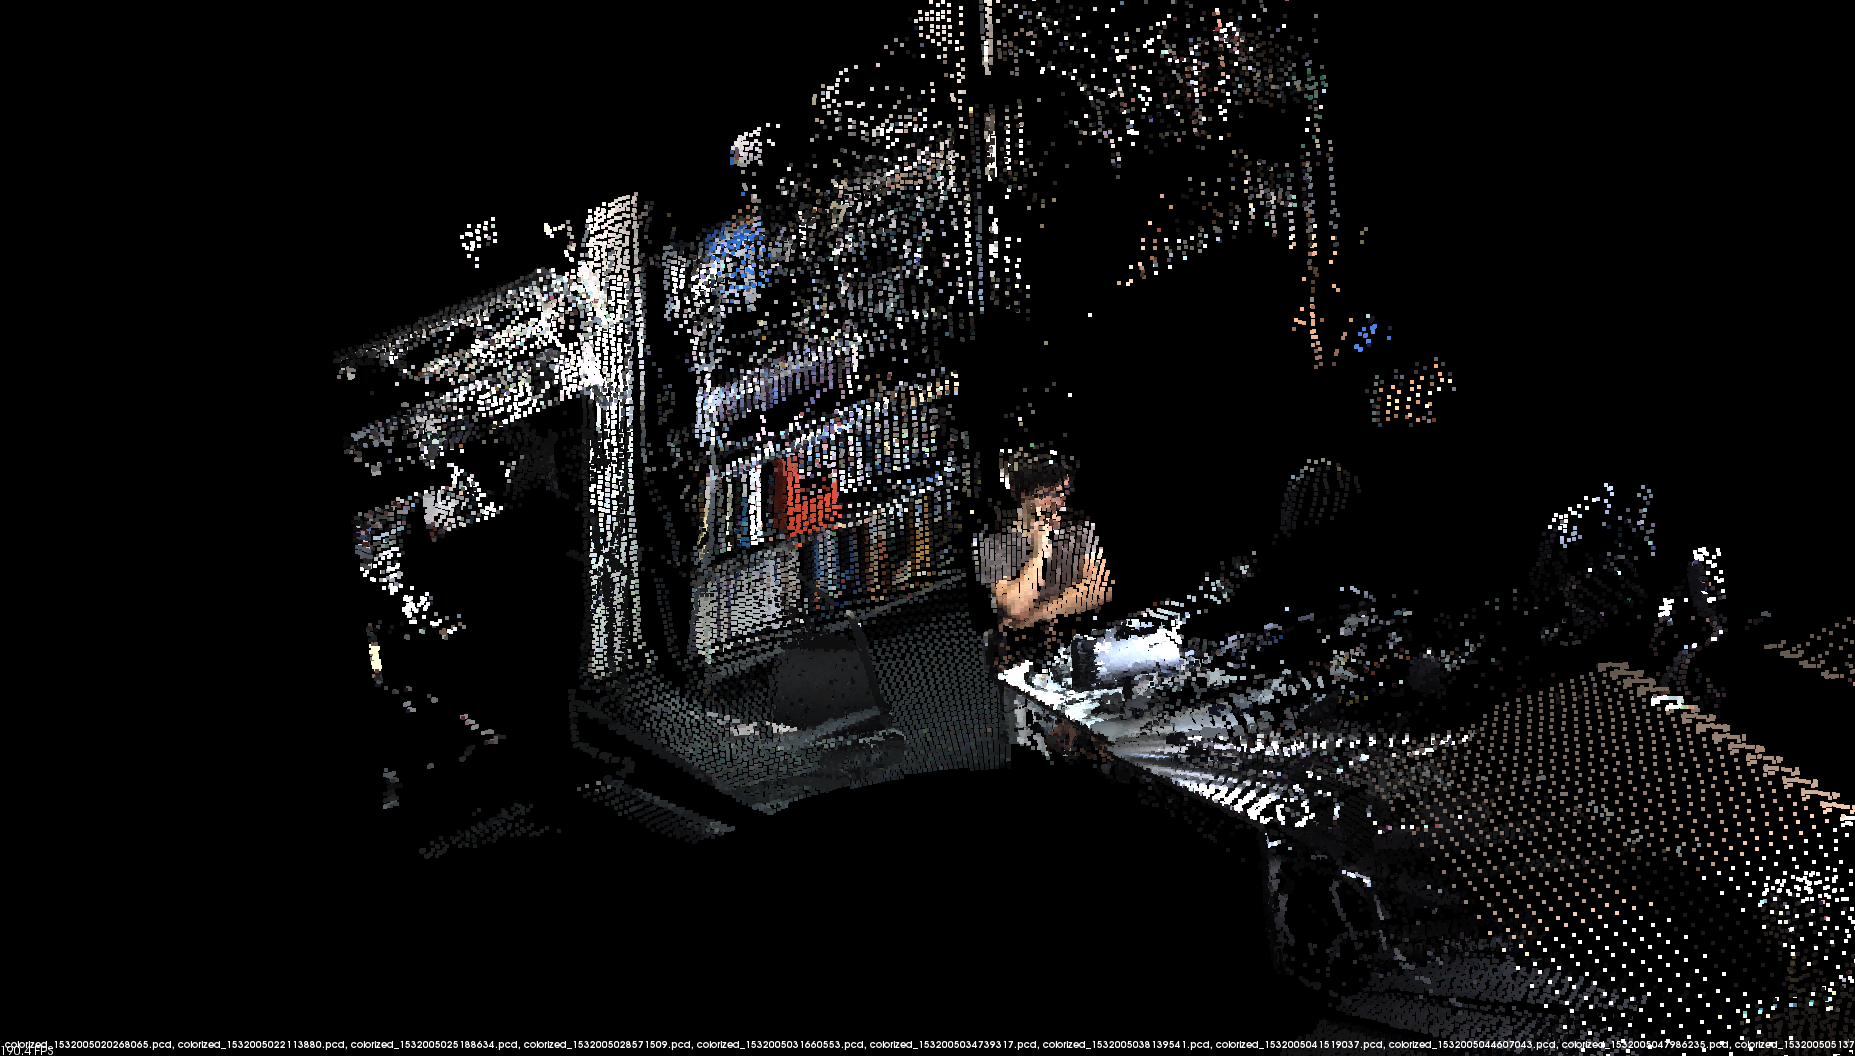
\includegraphics[width=\textwidth]{img/radlocc_medium_regist.png}
    \end{figure}

\end{frame}